\section{Proposed Solution}
    The proposed experimental setup\cite{gene2vecOFCLimpl}\cite{gene2vecimpl} mostly depends on the data collection and processing for a relatively straightforward neural network. The main components for the entire solution may be summarized in the \textit{mindmap} in Figure \ref{fig:mindmap}.
    % \begin{tikzpicture}
    % 	\path[mindmap,concept color=black,text=white]
    % 	  node[concept] {Computer Science}
    % 	  [clockwise from=0]
    % 	  % note that `sibling angle' can only be defined in
    % 	  % `level 1 concept/.append style={}'
    % 	  child[concept color=green!50!black] {
    % 		node[concept] {practical}
    % 		[clockwise from=90]
    % 		child { node[concept] {algorithms} }
    % 		child { node[concept] {data structures} }
    % 		child { node[concept] {pro\-gramming languages} }
    % 		child { node[concept] {software engineer\-ing} }
    % 	  }
    % 	  % note that the `concept color' is passed to the `child'(!)
    % 	  child[concept color=blue] {
    % 		node[concept] {applied}
    % 		[clockwise from=-30]
    % 		child { node[concept] {databases} }
    % 		child { node[concept] {WWW} }
    % 	  }
    % 	  child[concept color=red] { node[concept] {technical} }
    % 	  child[concept color=orange] { node[concept] {theoretical} };
    %   \end{tikzpicture}
    \begin{figure}
        \centering
        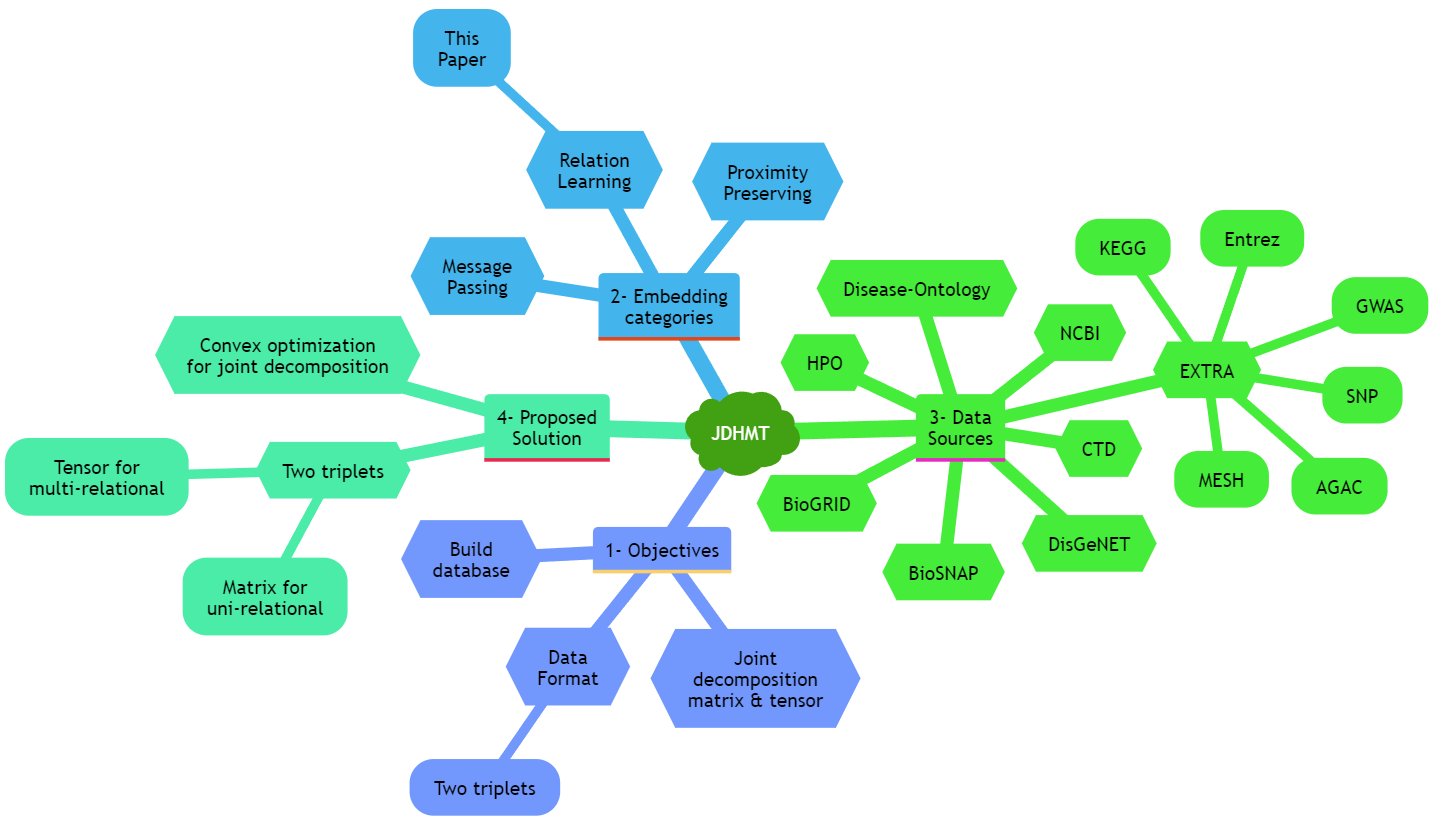
\includegraphics[width=180mm,scale=1]{mindmap.png}
        \caption{Mindmap}
        \label{fig:mindmap}
    \end{figure}

    The flow of the logic for each of the major components (viz., \textit{Data Collection}, \textit{Embedding Training}, \textit{Visualization} \& \textit{Downstream Task}) is described next:

    \subsection{Data Collection}

    The data sources are:
    \begin{enumerate}
        \item \textbf{GEO database}'s \textbf{GeneChip Human Genome U133 Plus 2.0 Array set},  which provides gene-expression information via the older micro-array based method. Probe sets with $\ge30$ samples and large intra-sample variance were chosen. The gene-coexpression was measured using the \textit{Pearson Correlation Coefficient}. The gene pairs with $\mathcal{PCC} \ge0.9$ were used for training
        \item Gene-gene interaction information is obtained from \textbf{Gene Ontology} annotations accessed via the \verb|R| package \verb|org.Hs.eg.db|. Gene pairs that share annotation (\textit{GO category "Biological Process"}) form the \textit{positive set} and those that don't, form the \textit{negative set}. The genes were also mapped to the \textbf{NCBI Entrez Gene} knowledge base.
        \item \textbf{GTEx v6} data was used to compute tissue specificity (\textit{z-score}) by comparing avg. gene expression of all genes across 27 tissues. Apparently, this value is mapped to the gene-expression info in (1) above
        \item With pathways information from \textbf{KEGG}, \textbf{Biocarta}, and \textbf{Reactome}, \textit{clusteredness} from \textbf{MSigDB pathways v5.1} is used to setup the \textit{Loss Function} for the optimization of the learnable parameters.
    \end{enumerate}

    \subsection{Embedding Training}

    In general, a neural embedding aims at mapping items in a discrete space into a continuous \textit{Euclidean} space. Embeddings enable the computation of \textit{gradients} and thus training of a neural network.

    /noindent There are two NLP methods, viz., \textit{skip-gram model} and \textit{continuous-bag-of-words}. Each can be quickly visualized using the following diagrams:

    First let us look at \textbf{\textit{skip-gram model}} (as in Figure \ref{fig:skipgram}): the target word is the input (\textit{here, it is "sat"}) and the model has to predict the most context sensitive words (excluding stop words) (\textit{here the words, "cat" and "mat"}). For this, the probabilities are predicted over entire vocabulary.\\

    \begin{figure}
        \centering
        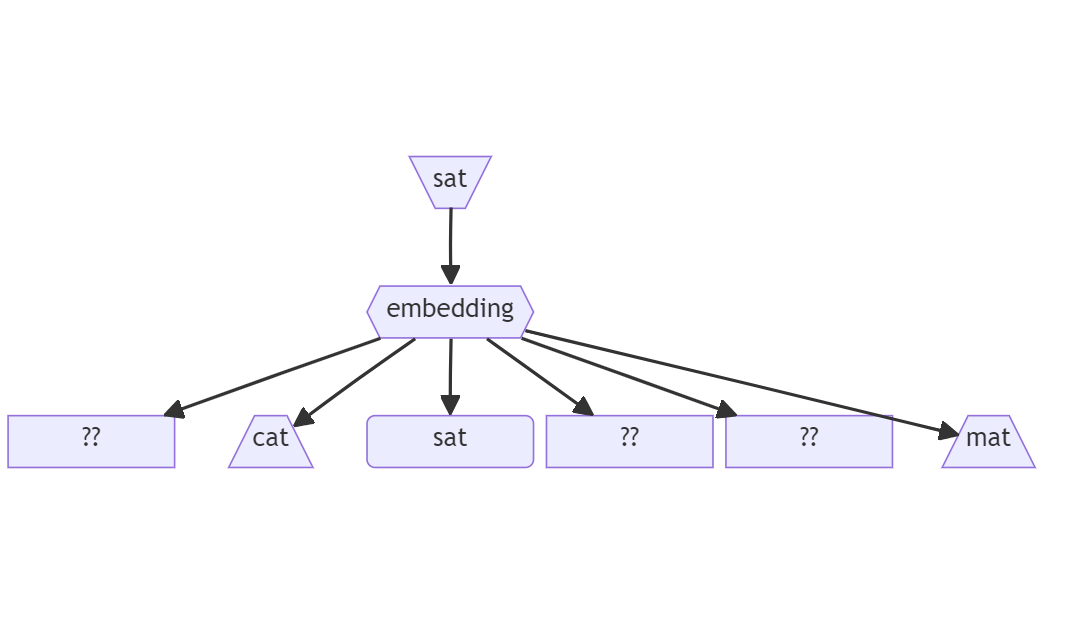
\includegraphics[width=140mm,scale=1]{skipgram.png}
        \caption{Skip-gram Model}
        \label{fig:skipgram}
    \end{figure}

    In the \textbf{\textit{continuous-bag-of-words model}} (as in Figure \ref{fig:cbow}): the context is the input, where the words preceding and following a target word are input, and a probability for the target word is predicted. In essence, it is just the reverse of \textit{skip-gram}.\\

    \begin{figure}
        \centering
        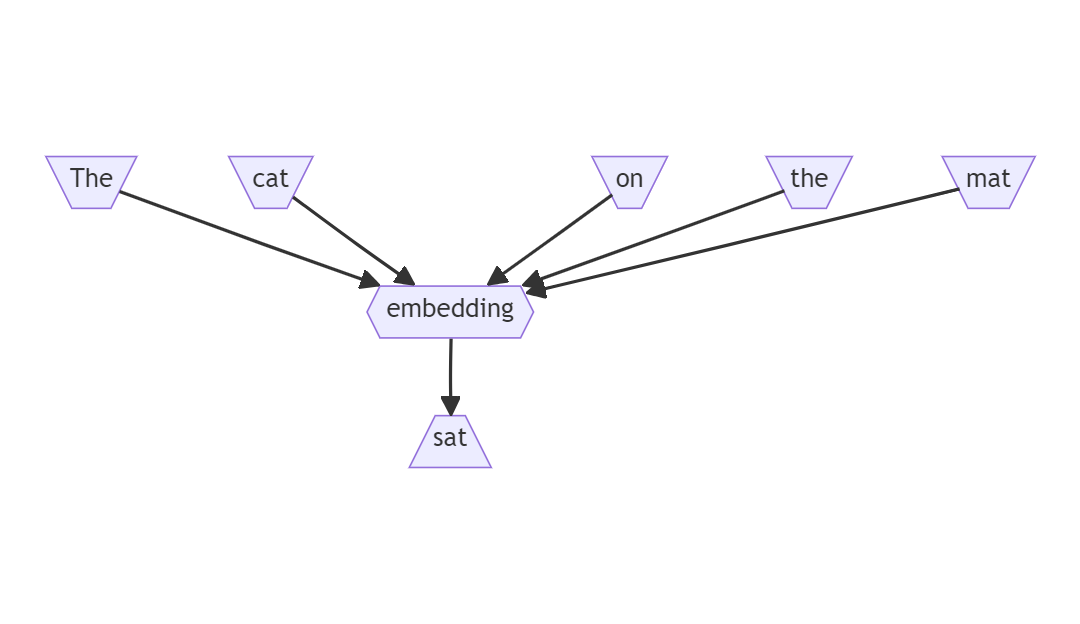
\includegraphics[width=140mm,scale=1]{cbow.png}
        \caption{Continuous Bag of Words Model}
        \label{fig:cbow}
    \end{figure}

    The \textbf{authors have used the \textit{skip-gram model} to model the learning}. The idea involves creating an ordered vocabulary of all unique genes, and represent each gene by a one-hot vector. These vectors are input to the neural network. The network calculates loss and thus gradients based on whether or not the correct probability of co-expression was predicted by the network. Further, a grid search is performed for hyper-parameters such as \textbf{\textit{number of iterations}} and \textbf{\textit{dimensions of embeddings}}.\\

    Once the parameters and hyper-parameters reach apparent convergence, the vector generated by the last hidden layer forms the gene embedding. The entire process may be understood as in the Figure \ref{fig:model}.

    \begin{figure}
        \centering
        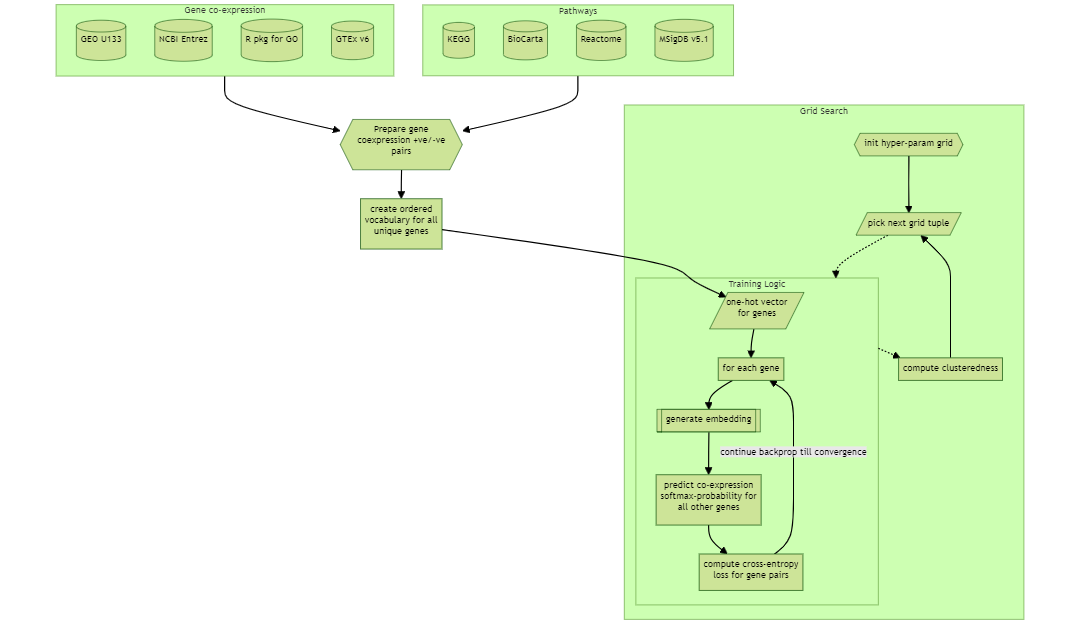
\includegraphics[width=205mm]{model.png}
        \caption{Embedding Training Logic}
        \label{fig:model}
    \end{figure}


    The cross-entropy loss attempts to minimize the following (\textit{as per the paper}):
    \begin{equation}
        -\sum_{(g_i, g_j)\in \mathit{T}} \mathit{Pr}(g_i | g_j)
    \end{equation}

    where,

    $\mathit{T:}$ set of highly co-expressed gene pairs

    $\mathit{Pr}(g_i | g_j)$ = $\frac{\mathit{exp(v_i^T v_j)}}{\sum_{j'} \mathit{exp(v_i^T v_{j'})}}$\\

    In other words, the cross-entropy loss will maximize the likelihood of highly co-expressed genes and reduce the likelihood of unrelated ones.

    \begin{mybox}
        This is my understanding. Seems the paper has some discrepancy in the formula though!
    \end{mybox}

    For the grid search that is used to find the most useful values for the hyper-parameter, the following clusteredness formula is used:

    \begin{equation}
        \mathit{clusteredness} = 
            \frac{
                \frac{1}{|Q|}
                \sum_{P\in Q}{
                    \frac{1}{\mathit{\#gene\,pairs\,in\,P}}
                    \sum_{g_i, g_j \in P}(v_{i}^{T}v_j)
                }
            }{
                \frac{1}{\mathit{\#gene\,pairs\,in\,Q'}}
                \sum_{g_i, g_j \in Q'}(v_{i}^{T}v_j)
            }
    \end{equation}
    
    where, the symbols have the following meaning:

    $\mathit{Q:}$ set of pathways in MSigDB (\textit{have co-expression})

    $\mathit{Q':}$ set of random gene pairs

    $g_i\in \mathbb{R}^d :$ one-hot vector for $i^{th}$ gene in ordered gene vocab of size $d$

    $v_i\in \mathbb{R}^k :$ embedding for the $i^{th}$ gene, of dimension $k$

    Further,

    $g_i$ and $v_i$ are related as: $v_i = W \cdot g_i$, \textit{where} $W \in \mathbb{R}^{d \times k}$ \textit{is the learnable parameter}.


    \subsection{Visualization by t-SNE}

    The authors utilize PCA to reduce the dimensionality of the generated gene embeddings and plot the t-SNE charts. The visual clusters are used for verifying the viability of the embeddings in terms of gene annotation similarity.

    \subsection{Predict Gn-Gn Ix}

    The downstream task of gene-gene interaction prediction is setup to establish the effectiveness of the generated embeddings in some real scenarios. 

    \begin{mybox}
        I am not delving into this experiment since that is not the focus of my study.
    \end{mybox}